\documentclass[twocolumn]{d-abst}
\usepackage[dvipdfmx]{graphicx}
\graphicspath{{figs/}}
% Add period after section number
\usepackage{secdot}
\sectiondot{section}

\title{脚車輪形態可変ロボットの構成法と環境適応形態遷移行動の実現}
\author{真壁佑,指導教員:稲葉雅幸}
\keywords{サーボモジュール,センサモジュール,車輪ロボット,形態変化,環境適応}

\begin{document}

\pagestyle{empty}
\maketitle
\thispagestyle{empty}
\sloppy

\section{はじめに}
近年,災害現場における救助や家庭環境での家事支援といった,人間の作業を代替するロボットに関する研究が行われている.
ヒューマノイドは脚による段差の移動や双腕による作業を行い,モバイルマニピュレータは室内での車輪を用いた高速な移動や荷物運搬を行うように,ロボットは動作環境に適した身体構成を持つが,人間のように広範囲に渡る環境で作業を達成するためにはハードウェアが環境に適した形に変化する必要がある.
%% しかし, 特定環境での動作達成を扱う多くのロボットとは異なり, 人間が行う作業は 1 つの環境だけでは完結せず, スーパーへの買い物のように屋内外にまたがる広い範囲での作業になるほど動作環境は多種多様になる.
%% そのため, 目標の性能を達成するためには自由度構成や利用する身体構造など,環境とタスクに対してハードウェアの最適化を行う余地がある.
これまで著者はロボットが多様な環境に適応する能力を拡張するために必要なハードウェア要素について研究を行っており,特に状況に応じて形態を変化させ最適な性能を発揮できるようなロボットの研究に取り組んでいる.

学士論文では筋骨格腱駆動ヒューマノイドの頭部に可動眼球を搭載し,高速な視点の変更動作と認識範囲の制御による効率的な環境認識システムを構築した.
このシステムにより,視界中の必要な領域のみで認識を行うことで,車両の周囲の効率的な安全確認と発進動作を達成した\cite{makabe2018eye}..
修士論文では車輪や駆動方式の変更が可能な関節を備え,状況に応じて形態を変化させるようなロボットに関する研究を進めている.
車輪を持つロボットについて,%% 環境中で移動能力に優れ継続した動作が可能なロボットの構成を目的として,上半身に筋骨格腱駆動の双腕を,下肢にインホイールモータを用いた倒立二輪を備えたロボットを構成した.
筋骨格腱駆動の双腕はハードウェア的に柔軟な構造を持つため環境接触を伴うタスクに向き,,倒立二輪の下肢は車輪による移動能力と制御的な安定性を備えるため,二つを組み合わせることで作業能力と移動能力を活用することが可能になロボットを構成した\cite{kawaharazuka2018twimp}.
駆動方式を変えることのできる関節について,動作中に関節の減速比を変えタスクに適した関節速度・トルクを発揮することを目的として,減速比可変で関節のロックも可能な関節を構成した.
%% この関節ではスリーブ式の変速機構を用いて,2段階の変速とスリーブを活用したロック機構を同一の機構で達成しており,30Nm程度の負荷がかかっている状態で関節の位置制御を切ること無く変速することに成功している.
また,開発した関節を腰に備えた三輪車型のロボットを構成し,物体の運搬タスクや三輪車型から倒立二輪型への遷移動作などを達成している\cite{makabe2019module}.

博士過程の研究計画では,修士まで行ってきた研究を発展させ,より多自由度なハードウェアにおける形態可変や,環境やタスクに対してアクチュエータ・センサ配置を最適化するようなシステムの構築を目指す.
そのために,共通の通信系を持つ身体構成要素の開発,身体構造可変な統合ハードウェア構造の生成,環境とタスクに対して最適な身体形態の探索と実現の3つの要素に分割して研究を進める予定である.

%% それに向けて,市販のシリアルサーボやリンク部品と自作のセンサ基板を組み合わせた脚車輪形態可変ロボットの構成に取り組んでおり,自由度の多い複雑な身体における形態変化手法の確立や,規格化されたアクチュエータ・センサ・リンクモジュールを用いた身体構造の自動生成

\section{研究概要・研究計画}

\subsection{学士論文:可動眼球を用いた認識制御と車両操作}

\begin{figure}[tbh]
 \begin{center}
  \begin{minipage}{0.8\columnwidth}
   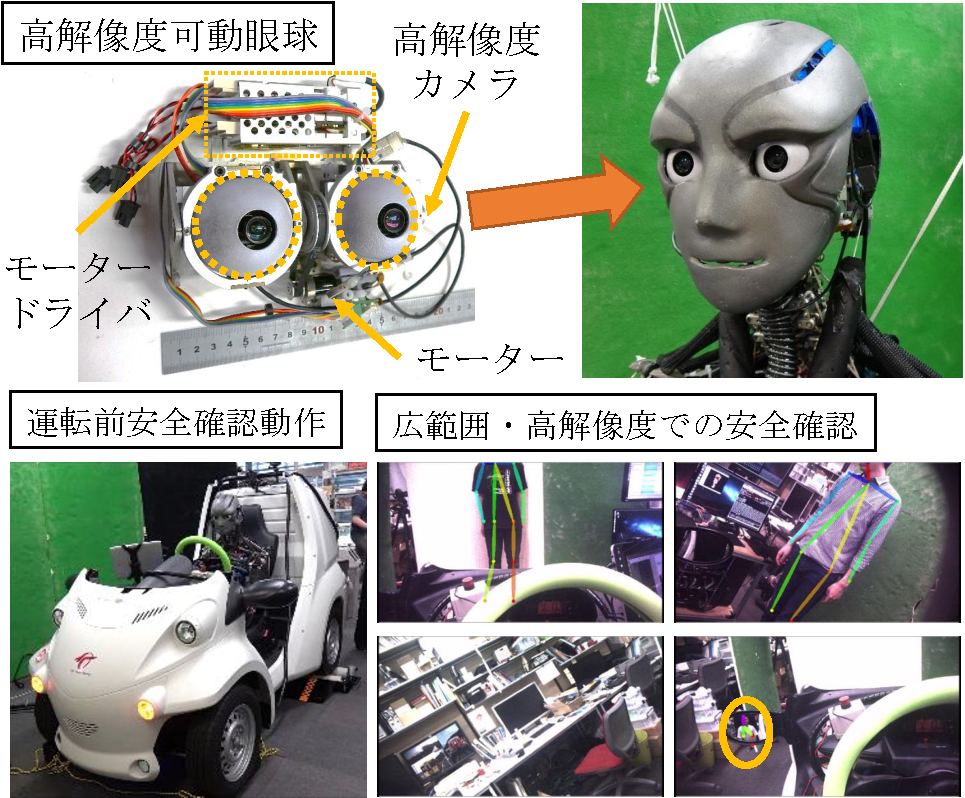
\includegraphics[width=\columnwidth]{1_eye.pdf}
   \caption{可動眼球を用いた認識制御と運転操作.}
  \end{minipage}
  \label{figure:nowprinting}
 \end{center}
\end{figure}

\subsubsection{高解像度な可動眼球視覚モジュールの構成}
生物が持つ可動する眼球には,高速に視野範囲を変更できる,動く物体を追従しつつ視野範囲を絞った効率的な認識を行えるといった利点が存在すると考え,両眼に4Kカメラを備え共通のtilt自由度と独立のpan自由度を持つ視覚モジュールを構成した.
眼球の自由度を環境認識行動に重要なものに絞り,小型で高解像度なカメラを用いることで,ヒューマノイドの頭部に収まるサイズの可動眼球を構成し,眼球の自由度を用いた高速な視点の変更動作を実現した.

\subsubsection{認識範囲の制御と車両操作への応用}
タスクに応じて画像処理を行う範囲を動的に変更することで効率的に環境認識を行える視覚システムの構成法について検証した.
また,環境認識動作の応用例として運転操作を行い,高解像度なカメラを用いたサイドミラーに映る小さな人物に対する注視動作により,人間と同様の視覚を利用した車両周囲の安全確認動作を実現した.%% 更に, 本可動眼球ハードウェアは視覚を用いたマニピュレーション研究に活用されている他, モジュラー型筋骨格プラットフォームにも搭載されており, 可動視覚と自己身体認識を用いた双眼による距離認識機能の獲得などの関連研究に広く利用されている.

\subsection{修士論文:環境適応可能な脚車輪ロボットの構成法}

\subsubsection{環境接触行動に適した筋骨格型倒立二輪ロボット}

\begin{figure}[tbh]
 \begin{center}
  \begin{minipage}{0.8\columnwidth}
   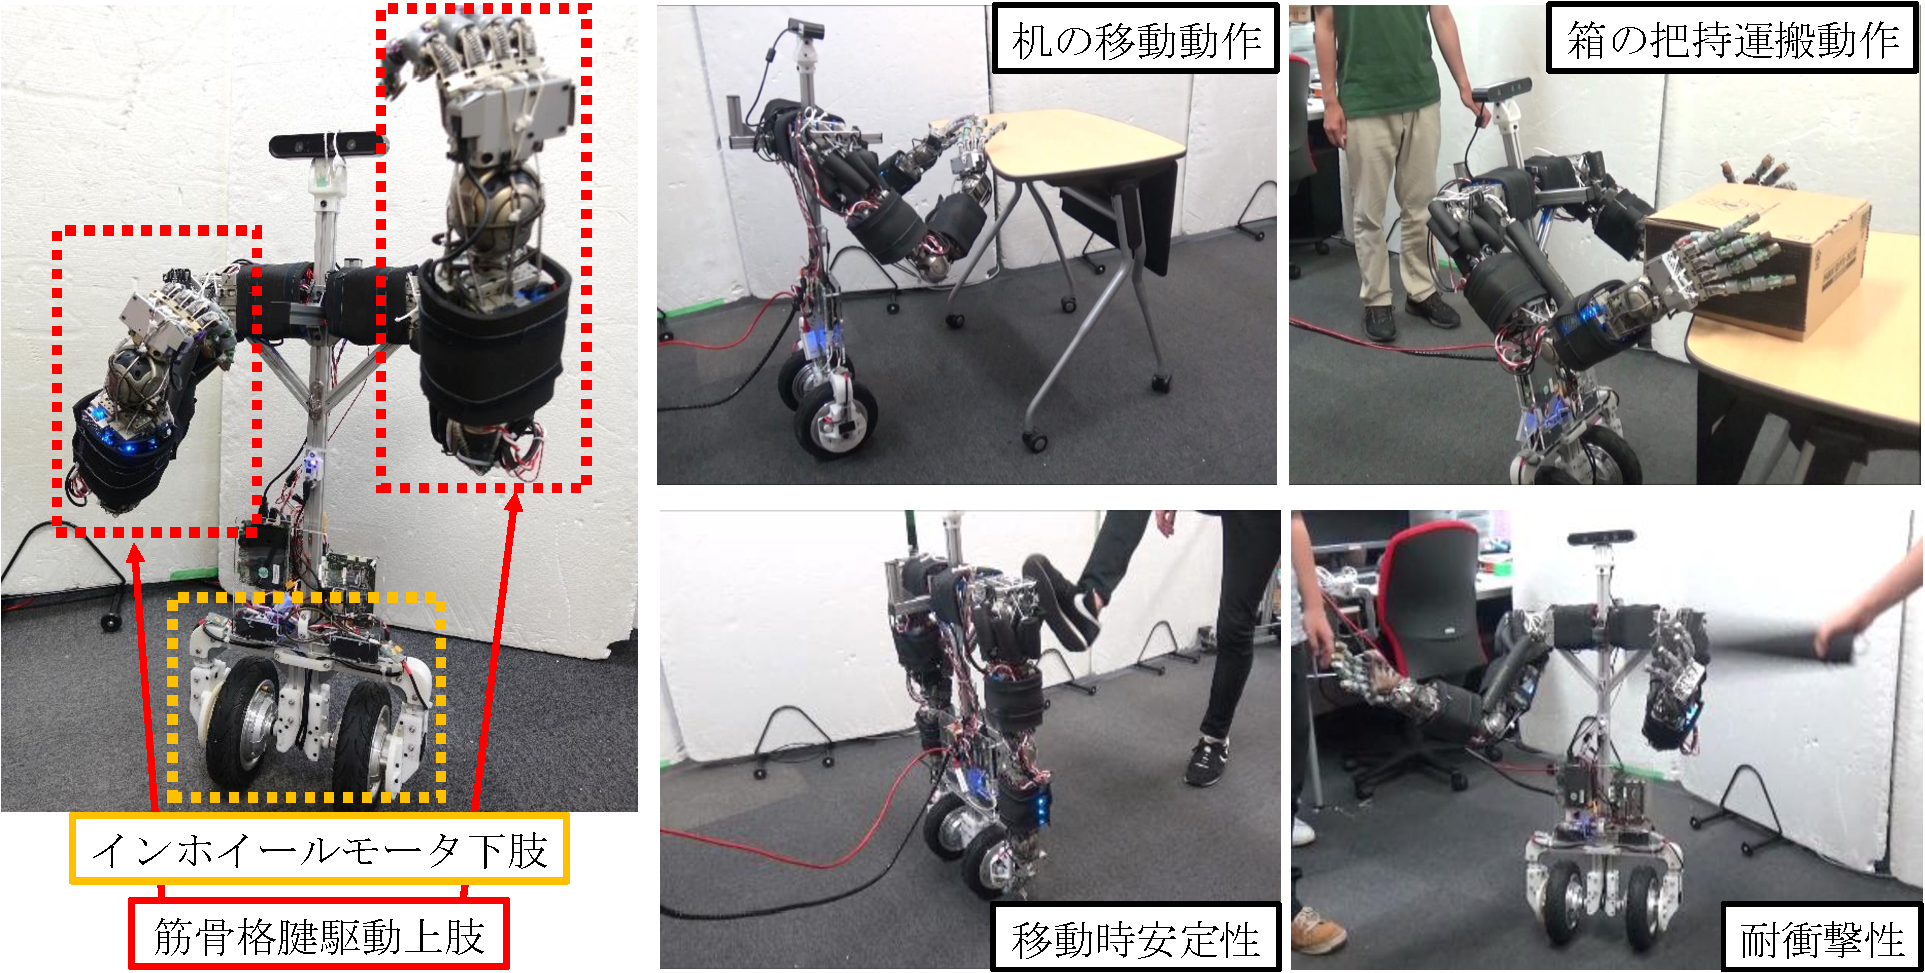
\includegraphics[width=\columnwidth]{2_twimp.pdf}
   \caption{環境接触行動に適した筋骨格型倒立二輪ロボット.}
  \end{minipage}
  \label{figure:nowprinting}
 \end{center}
\end{figure}

筋骨格腱駆動ロボットは柔軟な筋によって駆動される多自由度のリンク構造を持ち,関節の力制御が可能なため,環境との接触を伴う行動生成に向く.
また,モバイルマニピュレータは移動性能に優れ日常生活における家事タスクに関する研究が広く行われており,中でも倒立二輪型の足回りを採用し,小さなフットプリントと高い移動性能を持つものも存在する.
そこで,筋骨格腱駆動型の上肢構造と,倒立二輪型の下肢構造を組み合わせることで,実環境で接触を伴う動作を行う能力と多様な環境下での移動性能を併せ持つロボットを構成した.
上肢構造は筋骨格腱駆動構造によるハードウェア的な柔軟性を持ち,非線形弾性要素と拮抗腱駆動構造による関節トルク・剛性可変制御が可能なため,環境接触行動時の厳密な接触条件の計画が不要である.
%% 加えて, 関節の自由度よりも多い冗長な自由度を持つため, 動作中に筋が破損した場合でも作業を継続することができる. 
これらの特徴を活用し,環境接触動作として机の移動動作や,箱の把持運搬動作,壁への衝突時の衝撃緩和・転倒回避動作を実現した.
下肢構造は移動性能に加えて倒立二輪構造による姿勢安定性能を併せ持ち,並進・回転移動動作や,蹴り飛ばし時の転倒回避動作を達成した.
本ロボットは環境接触能力と冗長な自由度,移動能力を併せ持つことで,動作中に転倒しても故障しにくく動作を継続することが可能であり,環境中で繰り替えし動作を行い,成功と失敗を繰り返して動作を学習していくロボットに関する研究が行えるようになる.
加えて,筋骨格腱駆動ロボットの複雑な身体構造を制御するために筋長,筋張力,関節角度の対応を学習する研究において,上肢は(1)筋を駆動するアクチュエータモジュールと(2)関節角度検知可能な関節モジュール,(3)汎用フレームの三種を組み合わせて用意に構造を改変できる構造を持つため,特定の身体形状での学習結果を他の身体形状にも適用して容易に実験することが可能である.%% 上記の二点の特徴から, 本ロボットは学習型制御を行う研究プラットフォームとして優れている.

\subsubsection{可変減速関節ロック機構による関節機能の改変}

\begin{figure}[tbh]
 \begin{center}
  \begin{minipage}{0.8\columnwidth}
   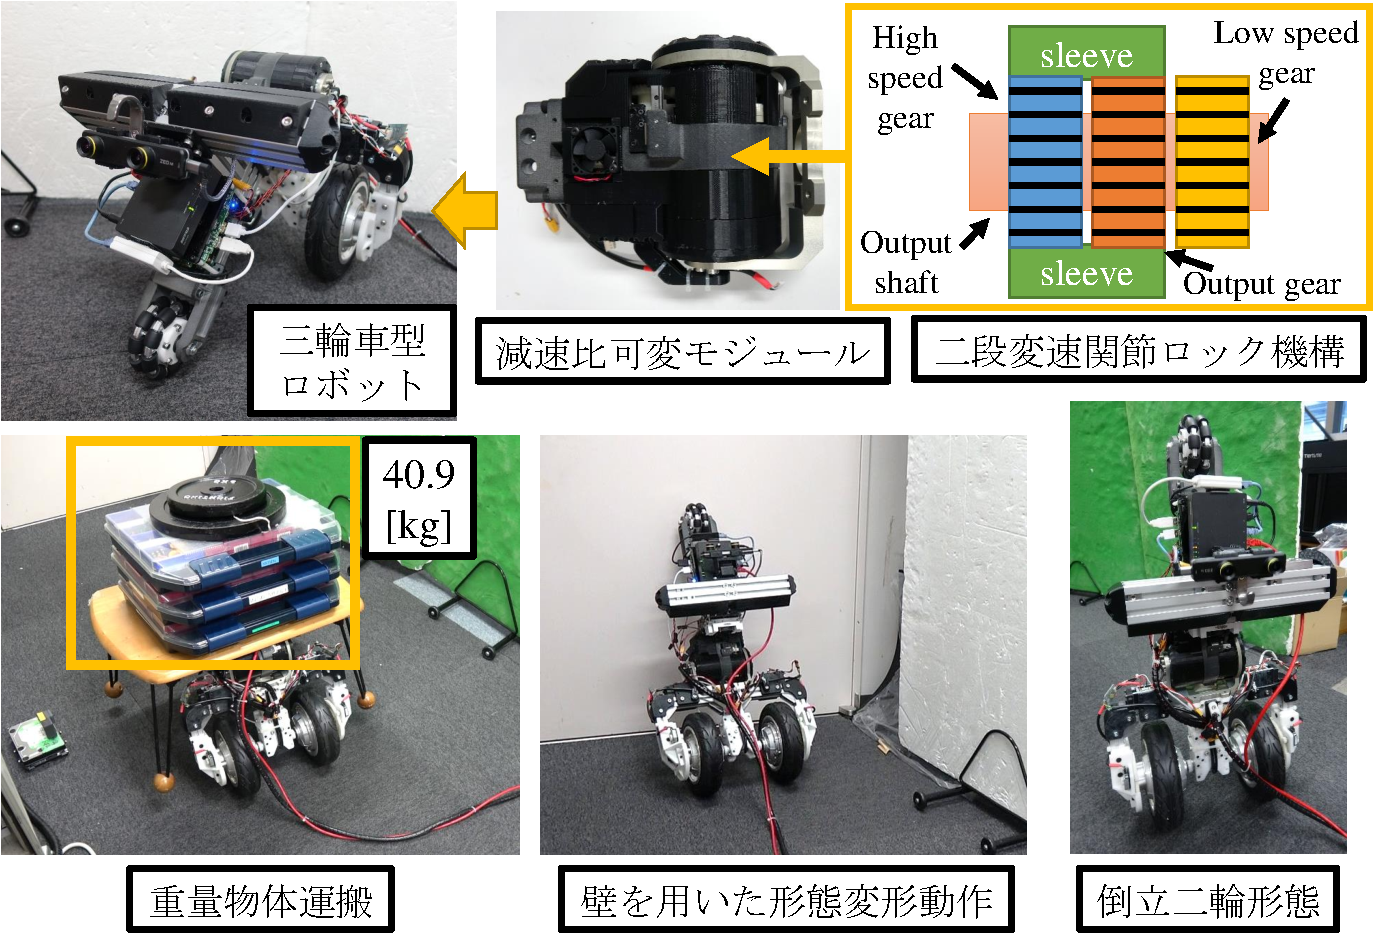
\includegraphics[width=\columnwidth]{3_module.pdf}
   \caption{可変減速関節と移動ロボットへの応用.}
  \end{minipage}
  \label{figure:nowprinting}
 \end{center}
\end{figure}

ロボットは必要なトルクと関節速度に最適化したモータと減速機構を有するが,作業中に必要なトルクや速度が不足した場合,故障やタスクの失敗の原因となる.
タスクに十分なトルクと速度を発揮するために,減速比の二段階変速機能と関節のロック機能を併せ持つ関節モジュールを開発した.
本モジュールは減速比を変えることで,負荷に耐えることのできる大トルクな関節と,環境接触時になじむことのできるバックドライバブルな関節の二つの機能を切り替えることができる.
更に,関節のロック機構を用いて電源を入れることなく自由度を固定し,タスク中の大負荷に耐えることのできる高剛性な関節に変化することも可能である.
開発した関節モジュールの評価のため,腰に関節モジュールを備え,倒立二輪での動作も可能な三輪車型ロボットを構成し,関節の駆動状態変更を活用した40.9kgの荷物の運搬と壁を用いた三輪車形態と倒立二輪形態の間で双方向の動作形態の遷移を達成した.

\subsubsection{共通の通信系を持つセンサ・アクチュエータによる脚車輪ロボットの構成と形態遷移動作}
多自由度かつ様々な形態に変化できるロボットの構成を目的として,市販のシリアルサーボやリンク部品と,自作のセンサ基板を組み合わせた脚車輪形態可変ロボットの構成に取り組んでおり,車両形態と人型形態の間での形態遷移動作や,歩行・走行動作を達成出来ている.
自作センサ基板について,市販のリンク接続部品と同様のサイズを持ち,シリアルサーボと同様の通信系を備え,設計の自由度が高く様々な構成の試作が可能になるため,後述する博士過程における研究のプラットフォームとして活用する予定である.

\subsection{博士過程の研究計画}
博士過程では,ロボットが環境やタスクに適した性能を発揮できる形態に変化することを目的として,アクチュエータ・センサ配置を最適化することが可能なロボットシステムの構築のために,以下の3つの実現を目指す.
\begin{itemize}
\item 共通の通信系と接続部を持つ身体構成要素の開発
\item 身体構造可変な統合ハードウェア構造の生成
\item 環境とタスクに対して最適な身体形態の探索と実現
\end{itemize}

\begin{figure}[tbh]
 \begin{center}
  \begin{minipage}{1.0\columnwidth}
    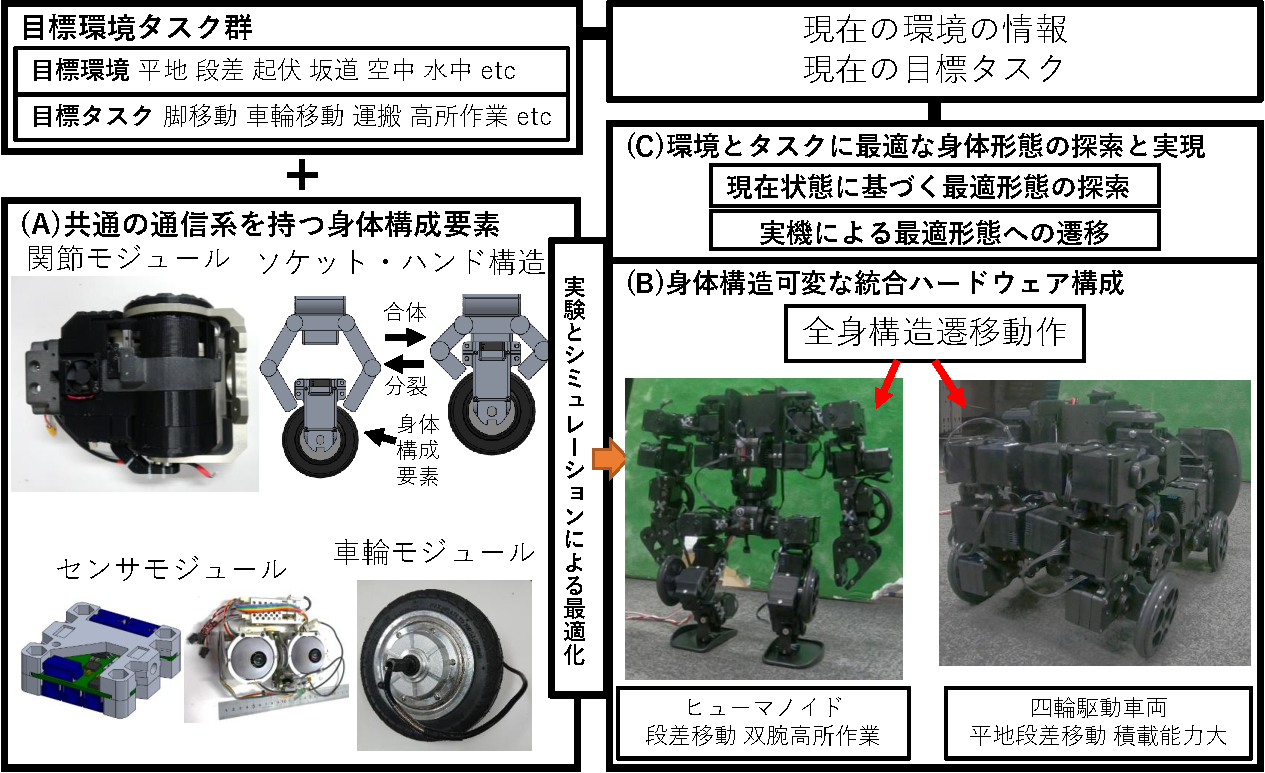
\includegraphics[width=\columnwidth]{4_matome.pdf}
   \caption{身体脱着構造可変ロボットの構成法と適応構成最適化.}
  \end{minipage}
  \label{figure:nowprinting}
 \end{center}
\end{figure}

\subsubsection{身体脱着構造可変ロボットの構成法と適応構成最適化}
身体構造の自動生成や構造改変の自由度を向上させるためには,機械的・電気的に構造の改変が容易な身体構成要素が必要であるため,センサとアクチュエータによらず共通の通信系や接続部を採用することが望ましい.
ここで述べている身体構成要素としては,身体を駆動する関節・リンクや,視覚や触覚などのセンサ,推力を発生させるための車輪やプロペラ,構成要素を脱着するためのハンドなどを想定しており,全体の重量や防水性能といったスペックに応じて適応が可能な環境がより広くなると考えている.
また,それらの要素を組み合わせて複合的な環境・タスクに適応できる統合的なハードウェアを構成するために,環境を仮定したシミュレータを用いてセンサおよびアクチュエータの配置や種類を最適化するための手法の構築が必要である.
この際,構成に用いた検証手法や実機実験の結果の中で,仮定した環境やタスクに依存しない一般性を見出すことで,一般的な身体構成の最適化指標の策定を目指す.
さらに,タスクを行っている最中に適切な身体構成を選択して形態遷移を達成するためには,タスクの達成時間や移動時の安定性といった最適化指標に基づく最適な形態の探索や,実機による多様な環境での形態遷移が必要となる.
また,大規模な姿勢遷移や構造改変を達成するためには,転倒回避のための指示領域の遷移計画や,関節負荷の低減のためのの発揮トルクの最適化を行う必要があると考えられる.
以上について,修士研究で利用しているハードウェアシステムを活用しつつ研究を進める計画である.

\section{おわりに}
著者はロボットが多様な環境に適応する能力を拡張するために必要なハードウェア要素について研究を行っており,今後の修士研究では多自由度な脚車輪ロボットによるセンサ情報を考慮した形態遷移動作に取り組む予定である.
さらに,規格化されたハードウェア要素を活用した身体構成の生成手法に関して新しく取り組む予定であり,多様な環境・タスク群に対して適した形態に変化できるロボットシステムの構築に向けて研究を進めることを検討している.

\bibliographystyle{d-abst}
\bibliography{main}

\end{document}

